\clearpage{\pagestyle{empty}\cleardoublepage}
\chapter{Impianti di trattamento del gas naturale}\thispagestyle{empty}
\chaptermark{Trattamento gas naturale}
Il gas naturale in uscita dai pozzi di produzione è caratterizzato dalla presenza di idrocarburi e altre sostanze associate. Queste sostanze influenzano negativamente il potere calorifico superiore (\(PCS\)) e possono creare problemi in fase di trasporto in condotta come la formazione di idrati. Per ovviare a questi problemi il gas naturale deve essere sottoposto a una serie di trattamenti con l'obiettivo finale di avere un prodotto facilmente trasportabile in condotta e che garantisca dei valori di \(PCS\) in linea con le richieste delle società di distribuzione. La formazione di idrati è influenzata dalla presenza di acqua associata al gas naturale, per ovviare al problema si rendono necessari interventi di disidratazione spinta della corrente gassosa. Altri trattamenti sono legati al recupero degli idrocarburi condensati, sostanze acide o elementi inerti.
%Per trattamento di gas naturale si intende l'insieme delle operazioni utili alla riduzione o abbattimento dei componenti che possono incidere sul trasporto e sull'utilizzo ultimo della risorsa. Le reti di distribuzione su larga scala prevedono delle specifiche tecniche e i trattamenti sono mirati al fine di ottenere valori che rispettino questi criteri. La produzione di gas naturale è normalmente associata alla presenza di acqua, la quale può presentarsi in forma liquida o gassosa. Il trattamento della disidratazione è fondamentale al fine di impedire la formazione di idrati, composti solidi che possono danneggiare le condotte durante il trasporto. Altri trattamenti sono legati al recupero degli idrocarburi condensati, che si manifestano al cambiare delle condizione di pressione e temperatura in superficie, e alla presenza di elementi corrosivi e elementi inerti, che possono diminuire i rendimenti del gas naturale.
%Il trattamento definitivo del gas può essere preceduto da un trattamento provvisorio (\figref{fig:generaltreatment}), nel quale si riducono o si inibiscono momentaneamente gli effetti dei componenti indesiderati del gas. Solitamente si fa riferimento al trattamento provvisorio nel trasporto del gas prodotto dall'area pozzo alla centrale di trattamento.
%\begin{figure}[htbp]
%    \centering
%    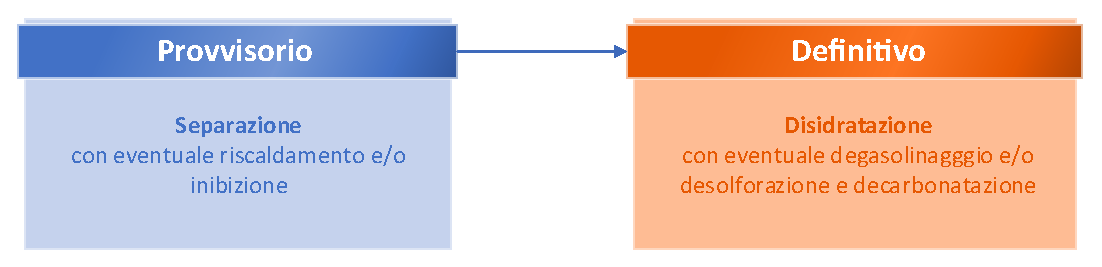
\includegraphics[width=\textwidth]{fig/impianti/generaltreatment.eps}
%    \caption{Tipologie di trattamento.}
%    \label{fig:generaltreatment}
%\end{figure}
Nel seguente capitolo si espongono le specifiche tecniche del gas, i processi di trattamento e le relative apparecchiature e impianti.

\section{Specifiche del gas di vendita}
Il gas naturale è una miscela di idrocarburi allo stato gassoso costituita in gran parte da metano e da idrocarburi più pesanti. Altre componenti spesso presenti sono acqua, anidride carbonica, azoto, idrogeno solforato e solfati, in alcuni casi anche elio e metalli pesanti come mercurio. In \tabref{tab:ng-composition} è riportato un esempio di composizione centesimale di un gas naturale. 

\begin{table}[htbp]
    \small
    \centering
    \caption{Composizione centesimale di un gas naturale tramite cromatografia del gas \parencite{mele2012produzione}.}
    \label{tab:ng-composition}
    \begin{tabular}{p{.45\textwidth}p{.45\textwidth}}
        \hline
        {\bf Componenti}                & {\textbf{\% in volume}}       \\ \hline
        Azoto                           & {0,17}                        \\
        Anidride carbonica              & {0,02}                        \\
        Metano                          & {99,71}                       \\
        Idrogeno solforato              & {-}                           \\
        Etano                           & {0,06}                        \\
        Propano                         & {0,03}                        \\
        Iso-butano                      & {0,01}                        \\
        Neopentano                      & tracce                        \\
        Iso-pentano                     & -                             \\
        Esani                           & -                             \\
        Ottani                          & -                             \\
        Eptani                          & -                             \\ \hline
    \end{tabular}
\end{table}

Ai fini della distribuzione e vendita, il gas naturale deve rispettare parametri specifici per poter poi essere immesso nelle reti nazionali. La rete di distribuzione non prevedono alcun trattamento del gas, ma delle semplici compressioni e decompressioni a seconda delle esigenze dell'utente finale. Il gas deve essere quindi opportunamente trattato nel rispetto di tali specifiche prima dell'immissione in rete.

\paragraph{Potere calorifico e indice di Wobbe}
Il gas naturale viene utilizzato maggiormente come combustibile e deve fornire un potere calorifico a specifica su tutto il territorio nazionale. Come parametro di riferimento si assume il potere calorifico superiore (\(PCS\)) standard pari a quello del metano pari a 9.100 kcal/Smc o 38,1 MJ/Smc, con un campo di variabilità nell'ordine del ±10\%. \'E importante ricordare che il \(PCS\) di un gas naturale può raggiungere questi valori anche in presenza di gas inerti come anidride carbonica e azoto, essendo formato da idrocarburi superiori che innalzano notevolmente il potere calorifico medio.\\
A questo proposito è utile introdurre l'indice di Wobbe \(I_W\) definito come:
\[I_w = \dfrac{PCS}{\sqrt{\rho_s}} \label{eq:wobbe} \]
dove \(\rho_s\) è la densità specifica del gas (densità relativa rispetto a quella dell'aria). L'indice di Wobbe di riferimento è pari a 11,6 kcal/Smc o 48,5 kJ/Smc, con una variabilità consentita del ±5\%. Nella valutazione della compatibilità di un gas per la sua immissione nella rete di distribuzione, è più corretto far riferimento all'indice di Wobbe: il campo di variazione più ristretto equivale a una minore presenza di gas inerti in miscela.

\paragraph{Punto di rugiada dell'acqua e degli idrocarburi}
Il gas non deve presentare condizioni di condensazione di acqua e/o idrocarburi in alcuna fase di trasporto e distribuzione. Le specifiche di immissione di pressione e temperatura variano a seconda dello specifico punto di consegna in funzione delle diverse condizioni geografiche e climatiche, con queste anche i punti di rugiada (\textit{dew point}) in acqua e in idrocarburi. Questi valori sono calcolabili tramite la rappresentazione del diagramma di fase relativo. Si considerano due specifiche diverse (in acqua e in idrocarburi) per i motivi seguenti:
\begin{itemize}
    \item \textbf{formazione di idrati}: si deve tenere maggiormente in considerazione la condensazione d'acqua rispetto a quella di idrocarburi a causa della formazione di idrati in condotta (trattati più avanti nel paragrafo ~\ref{section:dehidratation});
    \item \textbf{andamento non univoco della saturazione rispetto alla pressione}: essendo il gas naturale una miscela multicomponente, nel definire la specifica di \textit{dew point} in idrocarburi non si fa riferimento, come in acqua, a una pressione prefissata, ma a tutto il campo i pressioni a partire da quella atmosferica. Il diagramma di fase di una miscela multifase, visibile in \figref{fig:phasediagram}, è caratterizzato dalla zona di condensazione retrograda: in questa condizione con una riduzione di pressione (a temperatura costante) gli idrocarburi condensano anziché evaporare.
\end{itemize}

\begin{figure}[htbp]
    \centering
    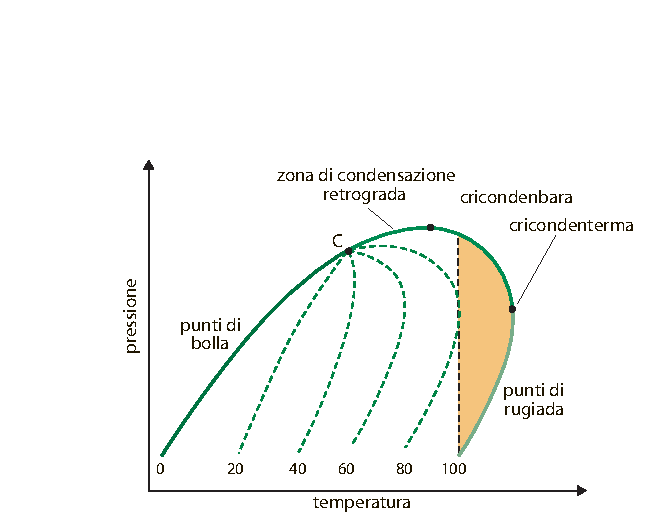
\includegraphics[width=.6\textwidth]{fig/impianti/phasediagram.eps}
    \caption{Diagramma di fase per una miscela multicomponente \parencite{bianco2005impiantigas}}
    \label{fig:phasediagram}
\end{figure}

\paragraph{Gas inerti (\ce{CO2} e \ce{N2})}
L'anidride carbonica (\ce{C O2}) in giacimento nasce dall'iterazione delle acque di strato con i silicati e i carbonati presenti. L'acido carbonico, composto che si forma per idratazione dell'anidride carbonica, rappresenta un problema concreto per gli impianti di trasporto del gas naturale.
\[\ce{H2O + CO2 -> H2CO3} \addtag \label{eq:acidocarbonico}\]
Oltre al problema degli acidi, la \ce{CO2} contribuisce all'incremento dei gas inerti totali (l'azoto \ce{N2} e appunto l'anidride carbonica). Si preferisce comunque rimuovere il \ce{CO2} (fino al raggiungimento dell'indice di Wobbe) rispetto all'azoto per la sua facilità tecnica di abbattimento. In generale si parla di volumi accettabili di \ce{CO2} attorno al 3\% con un contenuto totale di gas inerti che non deve mai superare il 6,5\%.

\paragraph{Acido solfidrico (\ce{H2S})}
L'acido solfidrico o idrogeno solforato (\ce{H2S}) è un gas incolore dall'odore caratteristico di uova in decomposizione. L'\ce{H2S} rappresenta uno dei sottoprodotti della decomposizione di proteine contenenti zolfo e dalla riduzione diretta di solfati (\ce{SO4^2-}) da parte di batteri, funghi e attinomiceti presenti in giacimento, ambiente anossico. L'\ce{H2S} è la principale causa di corrosione nella produzione di gas naturale, è altamente tossico e, a certe concentrazioni, anche mortale. Il contenuto massimo accettato è molto basso: Snam Rete Gas richiede un contenuto massimo di 6,6 mg/Smc.

\paragraph{Zolfo totale}
L'abbattimento dello zolfo totale nel gas naturale è legato più a questioni ambientali che a questioni di sicurezza. Il contenuto di zolfo totale massimo richiesto da Snam Rete Gas è di 150 mg/Smc, con un valore massimo di zolfo da mercaptani 15,5 mg/Smc. La rimozione dei mercaptani avviene tramite impianti che differiscono da quelli utilizzati per la rimozione di acido solfidrico e altri acidi.

\paragraph{Solidi sospesi}
I solidi sospesi vengono normalmente abbattuti durante i processi di separazione dei liquidi dal gas. Nel trattamento del gas naturale è sempre presente un sistema di filtraggio dei solidi sospesi prima del conteggio fiscale.

\begin{table}[htbp]
    \small
    \centering
    \caption{Parametri di controllo della qualità richiesti dalla Snam Rete Gas \parencite{snam2015codice}.}
    \label{tab:ng-specifiche}
    \begin{tabular}{p{.4\textwidth}p{.2\textwidth}p{.23\textwidth}}
        \hline 
        {\bf Parametri} & \multicolumn{1}{l}{{\bf Valori consentiti}} & {\bf Unità di misura} \\ \hline \hline
        Potere Calorifico Superiore & 34,95 ÷45,28 & MJ/Smc \\\hline
        Indice di Wobbe & 47,31÷52.33 & MJ/Smc \\\hline
        Densità relativa & 0.5548÷0,8 &  \\\hline
        Ossigeno & \(\leq\) 0,6 & \% mol \\\hline
        Punto di Rugiada dell'acqua (p=7 MPa) & \(\leq\) -5 & °C \\\hline
        Punto di Rugiada degli idrocarburi (p=0,1÷7 MPa) & \(\leq\) 0 & °C \\\hline
        Temperatura max & \textless 50 & °C \\\hline
        Solfuro di idrogeno & \(\leq\) 6,6 & mg/Smc \\\hline
        Zolfo da mercaptani & \(\leq\) 15,5 & mg/Smc \\\hline
        Zolfo Totale & \(\leq\) 150 & mg/Smc \\ \hline
    \end{tabular}
\end{table}

\section{Separazione gas-liquido}
La dinamica delle particelle disperse in un fluido studia i fenomeni di sedimentazione di gocce di liquido in un gas applicando gli stessi principi della separazione per gravità liquido-liquido. Il calcolo della velocità terminale \(w_t\) viene effettuato in base al bilancio statico delle forze che agiscono sulla singola particella, condizione nella quale la velocità è costante. Nel caso di particelle sferiche indeformabili di raggio \(D_p\), la velocità terminale \(w_t\) si può ricavare da:
\[w_t=\sqrt{\dfrac{4 \; g \; D_p(\rho_p-\rho_f)}{3 \; C_d \; \rho_l}} \addtag \label{eq:velterminale}\]
dove \(g\) è l'accelerazione di gravita, \(\rho_p\) e \(\rho_f\) sono la densità rispettivamente della particella e del fluido disperdente, \(C_d\) è definito coefficiente di galleggiamento o \textit{drag coefficient}. Nel caso di separazione per gravità liquido-liquido e condizioni di moto laminare, quindi per bassi valori del numero di Reynolds \(Re\), la \eqref{eq:velterminale} assume la forma della legge di Stoke:
\[w_t= \dfrac{(\rho_p-\rho_f)}{18\mu} \; D_p^2\; g \addtag \label{eq:stoke}\]
Per quanto riguarda particelle fluide immerse in un gas la condizione di moto laminare non è rispettata, a causa dei bassi valori della viscosità del gas quindi dell'alto valore del numero di Reynolds. In questo caso il calcolo del coefficiente di galleggiamento è effettuato tramite modelli sperimentali e calcolo per tentativi (\textit{trial and error}). La separazione per gravità è un processo grossolano che permette l'abbattimento di particelle nell'ordine di \SI{250}{\um} o di poco inferiore. Gli abbattitori (anche \textit{knockout} o KOD, \textit{Knock-Down Drum}) sono particolari separatori che agiscono per semplice gravità, utili per eliminare o solo l'acqua liquida o tutto il fluido trascinato dal gas. Sono generalmente collocati a monte di impianti di separazione meccanica a bassa temperatura (par. ~\ref{subsection:lts}) o a protezione di una fiaccola. Il dimensionamento dei KOD è basato sul bilancio tra tempo di ritenzione e tempo di decantazione delle particelle liquide in flusso gassoso.
Nei casi in cui si vogliano ottenere delle migliori performance di abbattimento dei liquidi si deve ricorrere a unità snebbianti che facilitino la coalescenza delle gocce e favoriscano l'abbattimento di gocce con diametro superiore ai \SI{10}{um}. Una delle unità snebbianti più comunemente utilizzate è il pacco rete (\textit{wire mesh pad}), inserito perpendicolarmente al flusso del gas. L'equazione che determina la velocità massima nella materassina snebbiante (\textit{mist eliminator}) è:
\[ w_t=K \sqrt{\dfrac{\rho_p-\rho_f}{\rho_f}} \addtag \label{eq:rete}\]
dove costante K varia in base al separatore e alla pressione operativa.\\
Nel campo della separazione di liquidi dal gas sono molto utilizzati anche i cicloni e i pacchi vani. I cicloni sono unità di coalescenza che sfruttano l'effetto centrifugo ottenuto tramite il movimento circolare del gas, con abbattimento delle particelle liquide fino ai \SI{3}{mu}. I pacchi di vani sono elementi coalescenti molto utilizzati anche nel trattamento dell'olio e sfruttano l'"effetto chicane" che si instaura nel flusso. Queste due unità di coalescenza sono preferite per il trattamento di gas caratterizzato da un notevole contenuto di solidi, come cristalli di paraffina separatisi dalla fase liquido in condizioni di bassa temperatura.

\section{Disidratazione e degasolinaggio} \label{section:dehidratation}
La variazione delle condizioni operative può dar luogo a fenomeni di condensazione di idrocarburi e/o acqua a partire da una miscela di idrocarburi allo stato gassoso. Quando in una corrente di gas naturale si ha la formazione di acqua libera, per determinate condizioni di flusso possono formarsi dei composti solidi detti idrati.
Il termine "idrato" è un termine generico per intendere nello specifico composti di inclusione o clatrati (dal latino \textit{clauthratus}, ingabbiato), strutture molecolari in cui un tipo di molecole avvolge un altro tipo di molecole. Le prime sono dette molecole ospitanti mentre le altre molecole ospiti. Per gli idrati di gas naturale le molecole ospitanti sono le molecole di acqua, mentre le molecole ospiti sono le molecole costituenti il gas naturale. La particolare conformazione è stabile in fase solida, dove le molecole ospitanti formano un reticolo cristallino al cui interno si generano della cavità in cui si posizionano le molecole di gas. 
A differenza del ghiaccio, la formazione degli idrati è fortemente dipendente dalle condizioni di pressione: maggiore è la pressione parziale del gas (quindi la concentrazione di molecole ospiti), maggiore è la temperatura di formazione degli idrati. La tendenza a formare idrati negli idrocarburi leggeri aumenta con il peso molecolare dell'idrocarburo e la presenza di anidride carbonica (\ce{CO2}) e solfuro di idrogeno (\ce{H2S}). 
In generale, affinché gli idrati si possano formare è necessario che si instaurino le seguenti condizioni:
\begin{itemize}
    \item presenza acqua allo stato liquido;
    \item presenza di idrocarburi;
    \item moto turbolento;
    \item relativamente alta pressione e bassa temperatura.
\end{itemize}
Sono stati sviluppati dei diagrammi che consentono di prevedere la formazione di idrati a determinate condizioni di pressione e temperatura, in funzione alla densità o peso molecolare medio del gas \figref{fig:formazioneidrati}.
\begin{figure}[htbp]
    \centering
    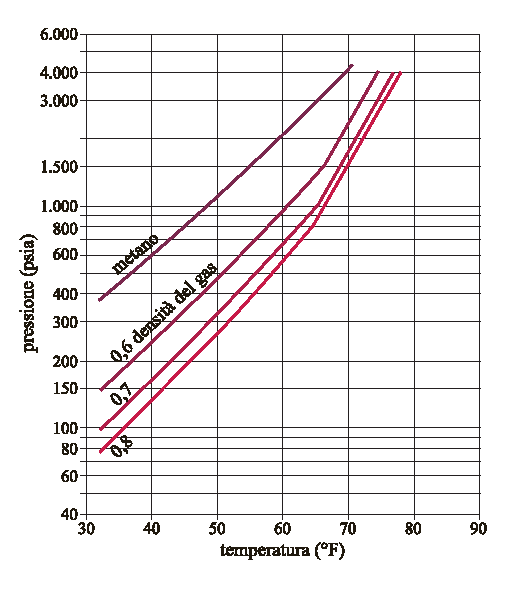
\includegraphics[width=.5\textwidth]{fig/impianti/formazioneidrati.eps}
    \caption{Diagramma della formazione degli idrati in funzione di temperatura e pressione \parencite{bianco2005impiantigas}.}
    \label{fig:formazioneidrati}
\end{figure}
Gli idrati possono formarsi all'interno delle singole condotte o concentrate su un collettore e possono danneggiare l'impianto in numerosi modi. L'occlusione parziale o totale della condotta porta a un aumento della pressione a monte del tappo di idrati con conseguente rottura della linea o per squarciamento della stessa o per impatto in corrispondenza di una curva (\figref{fig:idrati1}). Il tappo di idrati soggetto a riscaldamento localizzato può espandersi in modo incontrollato, portando all'inevitabile rottura della condotta (\figref{fig:idrati2}). Con l'interruzione di produzione a opera di una valvola, se la velocità del tappo è sufficientemente elevata, può intensificare gli effetti del colpo d'ariete  (\figref{fig:idrati3}).

\begin{figure}[htbp]
    \centering
    \subfloat[][Rottura per impatto di idrati su elemento curvo della condotta.]
    {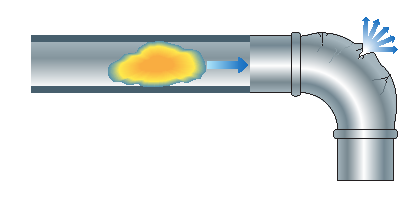
\includegraphics[width=.45\textwidth]{fig/impianti/idrati/idrati2.eps}  \label{fig:idrati1}} \qquad
    \subfloat[][Rottura per riscaldamento e espansione incontrollata.]
    {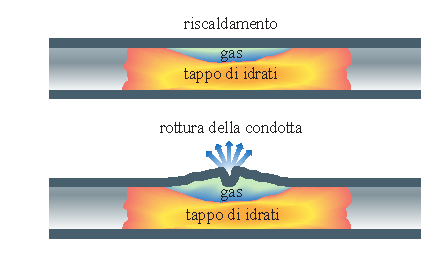
\includegraphics[width=.45\textwidth]{fig/impianti/idrati/idrati1.eps} \label{fig:idrati2}} \\
    \subfloat[][Rottura per inerzia del tappo di idrati.]
    {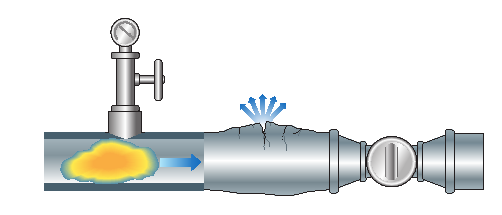
\includegraphics[width=.45\textwidth]{fig/impianti/idrati/idrati3.eps} \label{fig:idrati3}} 
\caption{Danni in condotta creati dalla formazione di idrati \parencite{borghi2005idrati}.}
\label{fig:idrati}
\end{figure}

Si inibisce la formazione di idrati in via temporanea aumentando la temperatura di trasporto del gas o tramite l'impiego di inibitori chimici, mentre in via del tutto definitiva con la completa disidratazione chimica.

\subsection{Inibizione chimica}
Gli inibitori vengono utilizzati per brevi tratti di linea, come i collegamenti tra le aree pozzo e le centrali di trattamento del gas naturale. Gli inibitori di idrati sono composti ad alta igroscopicità e possono agire in fase sia gassosa che liquida come l'alcol metilico (\ce{CH3-OH}), sia in fase solo liquida come il glicol monoetilenico o EG(\ce{C2H6O2}) e dietilenico o DEG (\ce{C4H10O3}). Il glicol è preferito all'alcol metilenico per la minore volatilità e infiammabilità.
Gli inibitori agiscono sul flusso gassoso in modo da abbassare il punto di congelamento spostando la formazione degli idrati verso valori più bassi di temperatura. La quantità o la concentrazione di glicol da iniettare è legata alle condizioni operative con cui si intende trasportare il gas naturale. La \figref{fig:inibizioneidrati} mostra l'abbassamento della temperature relativa alla curva di formazione degli idrati in funzione della concentrazione di EG disciolto in acqua.

\begin{figure}[htbp]
    \centering
    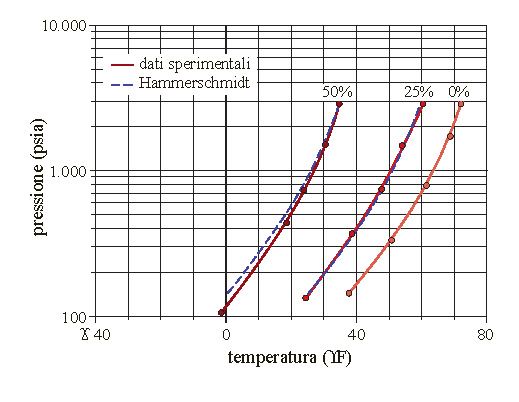
\includegraphics[width=.5\textwidth]{fig/impianti/inibizioneidrati.eps}
    \caption{Inibizione degli idrati tramite glicol etilenico \parencite{bianco2005impiantigas}.}
    \label{fig:inibizioneidrati}
\end{figure}

La rigenerazione del glicol, diluito in acqua all'arrivo della condotta, avviene tramite ebollizione dell'acqua in condensa, solitamente alla temperatura di 130°C.
%Mentre in passato l'inibizione degli idrati era un sistema impiegato spesso per il trasporto del gas naturale dalle aree pozzo alla centrale di trattamento, oggi si preferisce installare un sistema di disidratazione in prossimità del sito di produzione, soprattutto quando le condotte sono di notevole lunghezza.

\subsection{Disidratazione per raffreddamento} \label{subsection:lts}
Uno dei sistemi più semplici per la disidratazione di un gas consiste nel raffreddamento del gas stesso. La temperatura finale del trattamento deve coincidere con il punto di rugiada che si vuole ottenere. La disidratazione per raffreddamento, condizionamento a freddo o separazione a bassa temperatura (\textit{Low-Temperature Separation}, LTS) si ottiene sfruttando l'effetto Joule-Thomson: grazie alla semplice espansione, la corrente gassosa riesce a diminuire la propria temperatura senza l'ausilio di energia esterna. L'intero processo viene ottimizzato tramite uno scambio termico carica-effluente a opera di uno scambiatore gas-gas, tale da sfruttare le temperature raggiunte nel processo come punti di pre- e post-trattamento del gas naturale. Gli impianti LTS richiedono pozzi a gas ad alta pressione che garantiscano un sufficiente salto entalpico sulla valvola di laminazione. Le basse temperature permettono di ottenere un sensibile abbassamento del punto di rugiada del gas e un maggiore recupero di condensato rispetto ai separatori tradizionali. \\
Gli impianti di separazione a bassa temperatura (\figref{fig:lts}) si basano su due elementi di processo fondamentali:
\begin{itemize}
    \item separatore a bassa temperatura;
    \item scambiatore di calore.
\end{itemize}

\begin{figure}[htbp]
    \centering
    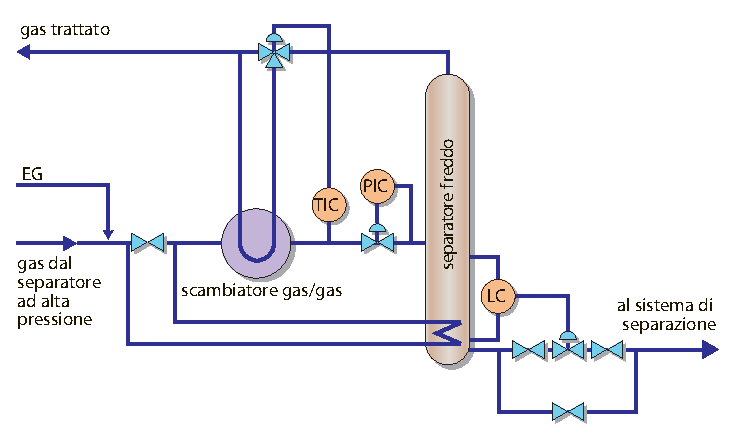
\includegraphics[width=.7\textwidth]{fig/impianti/lts.eps}
    \caption{Condizionamento del gas tramite separatore a bassa temperatura \parencite{bianco2005impiantigas}.}
    \label{fig:lts}
\end{figure}

Il separatore a bassa temperatura, anche detto separatore a freddo o a espansione, rappresenta il fulcro dell'impianto. Il gas viene immesso nella parte superiore del separatore tramite una duse. L'espansione del gas provocato dalla duse porta a una diminuzione repentina della temperatura del flusso con la condensazione di acqua. L'acqua, precipitando verso il basso, forma degli idrati che si raccolgono anche essi nella sezione inferiore per gravità. I liquidi e gli idrati vengono raccolti e scaldati tramite il gas in arrivo dal pozzo tramite una serpentina immersa. Questo riscaldamento viene effettuato per abbattere gli idrati e far rievaporare nuovamente i componenti leggeri come metano e etano. Il rendimento del processo dipende fortemente dalla temperatura finale raggiunta, perciò si consiglia di isolare i separatori a bassa temperatura per aumentare le performance di separazione per condensazione.
Lo scambiatore di calore gas-gas svolge una duplice funzione: provvede al preraffreddamento del gas in ingresso all'impianto di condensazione e al riscaldamento del gas in uscita riducendo al minimo la formazione di idrati. \\
L'unità di separazione a freddo può essere dotata di iniezione di inibitori al fine di abbassare ulteriormente la possibilità che si possano creare degli idrati al proprio interno. L'iniezione avviene a valle dell'espansione del gas e il sistema viene munito di un'unità di rigenerazione del glicol associato all'acqua in uscita.\\
Se le pressioni di arrivo del gas non sono sufficienti affinché l'espansione raggiunga temperature desiderate, l'impianto può essere aiutato da un ciclo di refrigerazione esterno a freon o propano. In questo caso si parlerà di disidratazione per raffreddamento con refrigerante o CRC (\textit{Compression Refrigeration Cycle}) e la temperatura di separazione viene ottenuta con uno scambiatore (\textit{chiller}) in cui il fluido refrigerante evapora a bassa temperatura e sottrae calore al gas da trattare. Le altre componenti dell'unità di trattamento non differisco dall'impianto LTS fin qui descritto.\\
Gli impianti di separazione a freddo sono impiegati non solo per la disidratazione del gas ma anche per il recupero degli idrocarburi superiori e pesanti in fase gassosa. Per la trattazione specifica si rimanda al paragrafo ~\ref{subsection:gasolina}.


\subsection{Disidratazione mediante assorbimento con glicol}
In questo tipo di disidratazione la tipologia di glicol più utilizzata è il trietilenico o TEG (\ce{C6H14O4}), anche se in alcuni casi può essere impiegato il DEG o l'EG. Il TEG è preferito agli altri per la più alta temperatura di decomposizione, importante ai fini della rigenerazione del glicol. La \figref{fig:disidratazioneglicol} mostra uno schema semplificato di impianto per la disidratazione con glicol.
\begin{figure}[htbp]
    \centering
    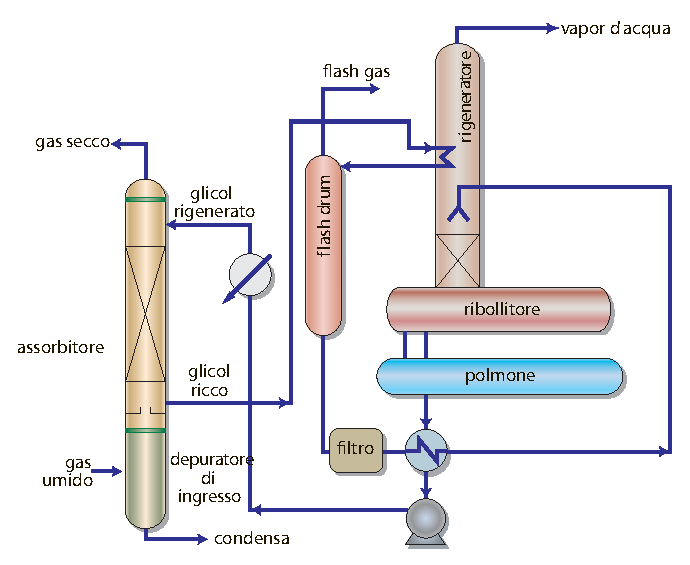
\includegraphics[width=.7\textwidth]{fig/impianti/deidratazioneglicol.eps}
    \caption{Schema semplificato di disidratazione con glicol \parencite{bianco2005impiantigas}.}
    \label{fig:disidratazioneglicol}
\end{figure}
Una corrente di TEG concentrato viene iniettata nella parte superiore della colonna di disidratazione, al fondo della quale viene fatto confluire il gas naturale da trattare. Il contatto col gas del glicol, altamente igroscopico, con più stadi di equilibrio in controcorrente porta alla disidratazione della corrente gassosa in uscita alla testa della colonna di assorbimento. Il TEG umido, cioè diluito in acqua, giunge al fondo della colonna e viene raccolto e inviato all'impianto di rigenerazione. Il recupero avviene tramite distillazione della soluzione.
La colonna di rigenerazione è divisa in due parti dalla sezione di alimentazione del glicol, dove la parte superiore è definita di rettifica, quella inferiore di arricchimento. Il TEG condensato viene preriscaldato tramite serpentina installata all'interno della colonna di rigenerazione, che funge da condensatore per abbattere le perdite di TEG. \\
Prima dell'immissione il TEG ricco viene convogliato in una camera di flash o \textit{flash drum}, nel quale i gas associati vengono recuperati tramite espansione a bassa pressione alla testa del separatore. \\
Dopo un eventuale passaggio tramite filtri a maglia e a carboni attivi, Il TEG ricco giunge alla colonna di rigenerazione, riscaldata tramite ribollitore di fondo solitamente di tipo \textit{kettle}. La temperatura del bollitore varia in funzione del tipo di glicol utilizzato: nel caso di utilizzo di TEG la temperatura è leggermente superiore ai 200°C in quanto ai 207°C il TEG tende a degradare, con DEG e EG le temperature operative scendono in quanto degradano attorno ai 165°C.\\
Per il riscaldamento si possono utilizzare vari sistemi (come tubi di fiamma e tubi di fumo immessi nel bagno da scaldare, fascio tubiero tradizionale, riscaldatore elettrico a resistenze corazzate, olio caldo (\textit{hot oil}), l'installazione deve avere comunque un occhio di riguardo sulla distribuzione della temperatura, ovvero il riscaldamento deve essere uniforme su tutta la superficie della camera di rigenerazione. \\
Il TEG rigenerato cede gran parte del calore passando nello scambiatore carica-effluente, viene pompato alla pressione di assorbimento e raffreddato alla testa della colonna di assorbimento.\\
Il trattamento continuo di disidratazione per glicol risulta essere molto semplice e il sistema di rigenerazione permette di raggiungere degli ottimi valori di concentrazione finale di TEG (solitamente attorno  al 98\%). Se si vogliono ottenere concentrazioni maggiori, occorrono dei processi di rigenerazione spinta con le quali i valori sono prossimi al 99,98\%. I processi di rigenerazione spinta più comuni sono l'installazione di colonna di \textit{stripping} con gas (\textit{dryer}), la rigenerazione sottovuoto (pressioni prossime a 0,1 bar) o i sisemi Drizo (utilizzo di gas di \textit{stripping} ottenuto vaporizzando composti liquidi mediante un adeguato serpentino di riscaldamento).

\subsection{Disidratazione mediante adsorbimento con setacci molecolari}
Nel caso in cui si voglia avere una disidratazione pressoché totale si può disidratare la corrente gassosa tramite adsorbimento a letto solido. L'acqua e alcuni inquinanti polari come \ce{CO2}, \ce{H2S} e mercaptani sono adsorbiti da zeoliti, cristalli altamente porosi appartenenti alla classe degli allumninosilicati. Essi hanno caratteristiche del tutto simili alle argille naturali: agiscono come un filtro molecolare (\textit{molecular sieve}), lasciando passare il gas e trattenendo le molecole polari. I cristalli di zeolite sono mischiati a dei leganti a base argillosa per ottenere i letti molecolari. L'adsorbimento è reversibile e i cristalli di zeolite possono essere rigenerati: le molecole adsorbite possono essere rilasciate in condizioni di alta temperatura o basse pressioni \parencite{grace2010techinf}. \\
Un tipico impianto di disidratazione è composto da due o più colonne di adsorbimento a setacci molecolari (solitamente tre, due in funzione e una in rigenerazione) e da un riscaldatore di gas di rigenerazione. L'adsorbimento di acqua si ottiene facendo confluire la corrente gassosa dall'alto verso il basso (\textit{down flow}) e il gas secco, in uscita dalla parte inferiore, viene immesso direttamente in rete. La rigenerazione dei setacci molecolari avviene tramite \textit{stripping}: il gas caldo di rigenerazione viene fatto fluire in senso opposto rispetto a quello di adsorbimento (\textit{up flow)}. L'aumento di temperatura consente la rimozione delle molecole polari adsorbite dai cristalli di zeolite e si associano alla corrente gassosa calda. Il gas di rigenerazione in uscita viene raffreddato e l'acqua viene separata per condensazione, mentre il gas viene riciclato verso i letti molecolari in funzione.\\
I setacci molecolari sono impiegati non solo per la disidratazione del gas ma anche per prodotti liquidi leggeri come GPL e condensati recuperati tramite LTS.

\begin{figure}[htbp]
    \centering
    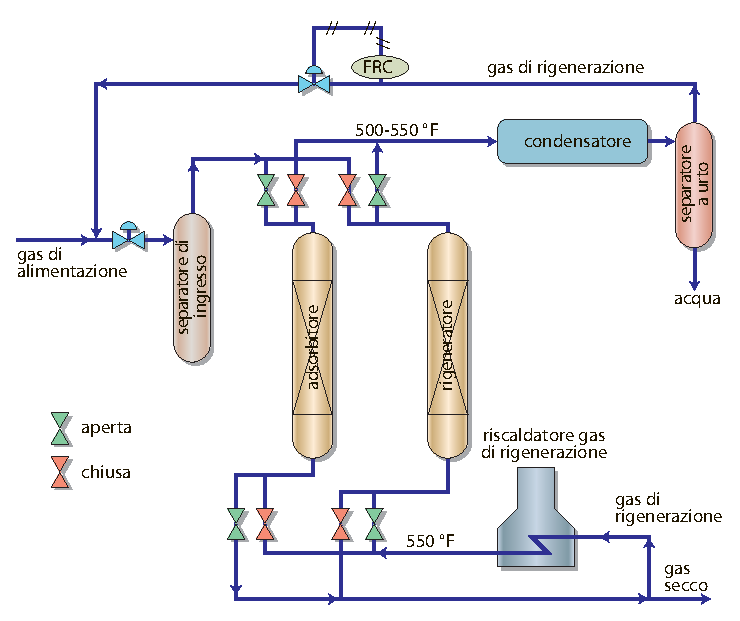
\includegraphics[width=.7\textwidth]{fig/impianti/molecularsieve.eps}
    \caption{Schema di disidratazione a due letti \parencite{bianco2005impiantigas}.}
    \label{fig:molecularsieve}
\end{figure}

\subsection{Degasolinaggio} \label{subsection:gasolina}
Il degasolinaggio viene effettuato per rispettare le specifiche del punto di rugiada degli idrocarburi, utili a garantire degli standard di trasporto nella rete di distribuzione. Il condensato, anche definito gasolina, è un liquido che si ricava dalle frazioni meno volatili del gas come propano, butano, pentano e altri idrocarburi superiori (\tabref{tab:gasoline-composition}). La composizione della gasolina varia notevolmente a seconda della provenienza: gas associato a greggio, gas da giacimento a gas condensato, gas da giacimenti a gas. La gasolina si trova in fase gassosa alle condizioni di giacimento e in fase liquida alle condizioni di superficie. Il suo aspetto è quello di benzina o petrolio leggero, il colore può variare dal bianco paglierino, all'azzurro e rossastro.
\begin{table}[htbp]
    \small
    \centering
    \caption{Composizione centesimale stimata di gasolina da gas naturale tramite distillazione \parencite{anderson1924composition}.}
    \label{tab:gasoline-composition}
    \begin{tabular}{p{.70\textwidth}p{.20\textwidth}}
        \hline
        {\bf Componenti}                & {\textbf{\% in volume}}       \\ \hline
        Propano e butano                & {20}                          \\
        Isopentano                      & {13}                          \\
        N-pentano                       & {17}                          \\
        Isoesano                        & {9}                           \\
        N-esano                         & {15}                          \\
        Isoeptano                       & {8}                           \\
        N-eptano                        & {12}                          \\
        Ottani                          & {4}                           \\
        Olio assorbito                  & {2}                           \\ \hline
    \end{tabular}
\end{table}
%Nel trattamento del gas proveniente da un giacimento di gas condensati il GOR (\textit{Gas Oil Ratio}) è molto alto e il gas associato è ricco di gas propano e butano e si realizza un terzo prodotto definito GPL, acronimo di gas di petrolio liquefatti (in inglese LPG, \textit{liquid petroleum gas}). Il GPL è una miscela di propano e butano con contenuti marginali di etano e di idrocarburi superiori e, in qualità di prodotto finito fruibile dall'utente finale, deve rispettare determinate specifiche tecniche. Lo stoccaggio del GPL per lunghi tempi (e.g. trasporto in mare) a pressione ambientale avviene tramite refrigerazione, per ridurre la volatilità e aumentare così la stabilità della miscela. 
Il processo più semplice e più impiegato per il degasolinaggio è basato sulla refrigerazione del gas. In particolare si fa riferimento alla separazione per raffreddamento per espansione (LTS) o per raffreddamento con refrigerante (CRC), impianti del tutto similari a quelli impiegati per la disidratazione.\\
Nell'unità di separazione a freddo il gas viene condensato mediate refrigerazione. Il processo è sempre bifase e la separazione acqua-idrocarburi (acqua eventualmente associata a glicol) avviene a valle tramite separatore bifase. In uscita dal separatore a freddo, l'acqua viene convogliata e trattata all'esterno mentre il condensato viene stabilizzato. La separazione gas-liquido a freddo in questo caso richiede sistemi di abbattimento delle goccioline più raffinati rispetto alla semplice materassina filtrante, poco indicata a causa della possibile formazione di cristalli di idrati e paraffina. L'impianto di separazione a freddo è indicato più per il trattamento dei condensati che per la semplice disidratazione poiché la variazione di fase degli idrocarburi, al contrario dell'acqua, risente delle condizioni di pressione.

\section{Altri trattamenti}
A seconda della composizione del gas di giacimento, il trattamento del gas naturale prevede ulteriori processi al fine di renderlo a specifica. \\
Il processo di addolcimento consiste nella rimozione dal gas naturale di gas acidi come \ce{CO2} e \ce{H2S} e consiste nell'assorbimento di tali sostanze mediante soluzioni alcaline. La reazione si basa quindi sulle reazioni di neutralizzazione tra acido debole e reagente basico. Requisito fondamentale del processo è la sua reversibilità. 
I reagenti più comunemente utilizzati sono le alcanolammine, ammine associate a gruppi alcanoli, gruppi alchilici o alcanoli a seconda che si tratti di un'ammina primaria, secondaria o terziaria. Le ammine accettano un protone sotto forma di ione idrogeno \ce{H+} tramite una reazione altamente esotermica. Trattandosi di fase liquida, il rendimento del processo di addolcimento dipende dalla velocità di reazione e dal passaggio della fase gassosa a quella liquida. La superficie di contatto tra le due fasi è proporzionale al rendimento di processo. La \figref{fig:ammine} mostra uno schema semplificato del trattamento di assorbimento con relativa rigenerazione delle alcanolammine. Il gas acido viene in contatto con la soluzione amminica e raffreddato nella colonna di assorbimento. Essendo la reazione altamente esotermica, le basse temperature favoriscono l'assorbimento. La soluzione al fondo della colonna viene convogliata in una camera di flash dove si separa parte del gas associato al liquido e la soluzione viene trasferita all'impianto di rigenerazione. Le alcanolammine sono rigenerate tramite stripping in corrente di vapore. Le ammine soffrono in modo particolare di degradazione termica, perciò la temperatura di rigenerazione è limitata e si preferisce l'utilizzo di soluzioni molto diluite.\\
\begin{figure}[htbp]
    \centering
    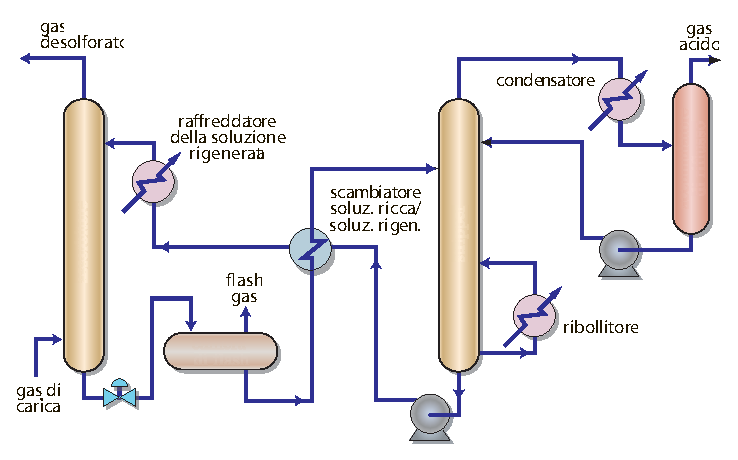
\includegraphics[width=.7\textwidth]{fig/impianti/ammine.eps}
    \caption{Lavaggio amminico \parencite{bianco2005impiantigas}.}
    \label{fig:ammine}
\end{figure}
L'addolcimento del gas può essere effettuato anche tramite soluzioni di carbonato potassico a caldo: al vantaggio del processo di assorbimento non esotermico (minor dispendio energetico dovuto al raffreddamento della colonna di assorbimento e minor esigenza di grandi superfici di scambio), si contrappone la necessità di reintegrare l'acqua che per alte temperature satura il gas trattato.\\
La rimozione parziale dei gas acidi al gas naturale si può ottenere tramite membrane semipermeabili: la corrente gassosa viene frazionata sulla base della permeabilità selettiva di alcuni composti polari rispetto agli idrocarburi.\\
Altri trattamenti che il gas naturale può subire sono il lavaggio del gas di coda, l'assorbimento fisico, la rimozione di \ce{H2S} tramite processi ossidativi, i filtri a carboni attivi.

\section{Apparecchiature di processo e impianti particolari}
I processi fin qui descritti possono realizzarsi tramite un impianto di trattamento, l'insieme delle infrastrutture utili a rendere il gas erogato dai giacimenti conforme ai requisiti di pressione, temperatura e qualità necessari all'immissione nella rete di distribuzione. L'impianto di trattamento è quindi progettato in base alle caratteristiche fisico-chimiche del gas naturale prodotto e alle specifiche di vendita. Nel seguente capitolo sono descritte le apparecchiature con le quali si realizzano i trattamenti richiesti.

\subsection{Separatori} %tesi+doc.ettore
I separatori sono gli apparecchi più utilizzati per la separazione di un flusso combinato liquido-gas dei suoi due componenti. I separatori sono classificati in base alla loro configurazione operativa:
\begin{itemize}
    \item \textbf{separatori orizzontali} (\figref{fig:corpo-singolo}): sono estremamente economici quando vengono trattati volumi importanti di gas. La disposizione orizzontale garantisce maggiori rendimenti rispetto a quella verticale per via del maggior tempo di permanenza delle goccioline nel separatore. Un separatore orizzontale a doppio corpo è definito \textit{slug-catcher} (\figref{fig:corpo-doppio}), con il corpo superiore completamente libero e il corpo inferiore che funge da polmone del liquido. La configurazione dello \textit{slug-catcher} permette di lavorare con alte portate e bruscamente variabili, a differenza del separatore singolo. I separatori a singolo o doppio corpo non sono particolarmente indicati per il trattamento di fluidi contenenti sabbia o fango, a causa della bassa capacità di eliminazione dei depositi e quindi l'accumulo degli stessi sul fondo;
    \item \textbf{separatori verticali} (\figref{fig:separatore-verticale}): nonostante le minori performance rispetto ai separatori orizzontali, sono comunque impiegati nell'ambito del trattamento del gas naturale quando i flussi sono caratterizzati da fango, sabbia o gas associato a olio. Inoltre, i separatori verticali sono preferiti in ambito off-shore, vista la scarsa disponibilità di spazio;
    \item \textbf{separatori sferici}: impiegati per la loro compattezza, i separatori sferici rappresentano un giusto compromesso tra i rendimenti di un separatore orizzontale e le ridotte dimensioni di ingombro del separatore verticale. Attualmente i separatori sferici sono poco impiegati in ambito tecnico-progettuale.
\end{itemize}
\begin{figure}[htbp]
    \centering
    \subfloat[][Separatore orizzontale a corpo singolo.]
    {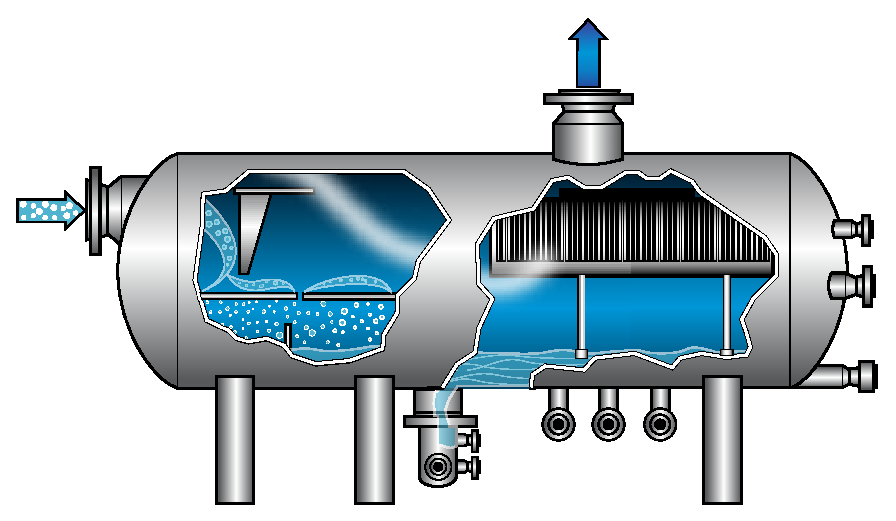
\includegraphics[width=.45\textwidth]{fig/impianti/separatori/horizontal-separator.eps}  \label{fig:corpo-singolo}} \qquad
    \subfloat[][Separatore orizzontale a doppio corpo o \textit{slug-catcher}.]
    {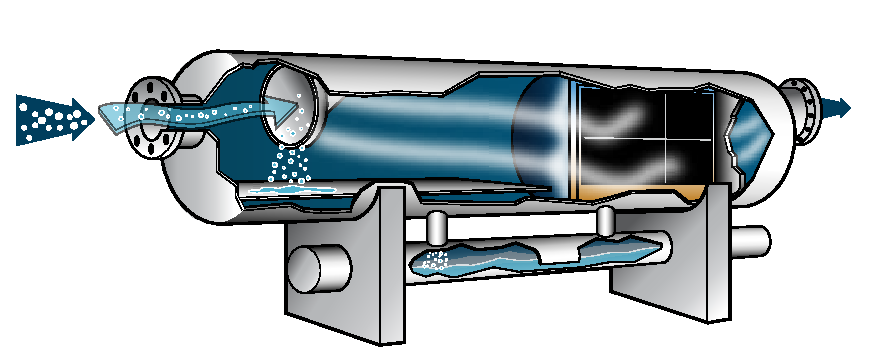
\includegraphics[width=.45\textwidth]{fig/impianti/separatori/double-barrel.eps} \label{fig:corpo-doppio}} \\
    \subfloat[][Separatore verticale.]
    {\makebox[.6\textwidth]{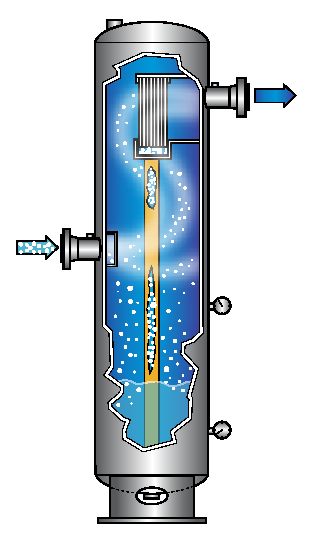
\includegraphics[height=.45\textwidth]{fig/impianti/separatori/vertical-separator.eps}} \label{fig:separatore-verticale}} 
\caption{Separatori orizzontali e verticali bifase dotati di dispositivi snebbianti \parencite{peerless2009vane}.}
\label{fig:bifase}
\end{figure}
I separatori possono essere forniti di elementi interni come deflettori, dighe, materassina snebbiante e/o pacco lamellare (\figref{fig:pacco-lamellare}) nel caso in cui si voglia aumentare la performance di separazione per semplice gravità. A seconda della configurazione i separatori possono separare la fase liquida dalla fase gassosa oppure riescono a operare una separazione spinta: si parla in questo caso di separatori bifase o separatori trifase (\figref{fig:trifase-interno}).
\begin{figure}[htbp]
    \centering
    \subfloat[][Vista interna di un separatore trifase dotato di pacco lamellare e materassina snebbiante.]
    {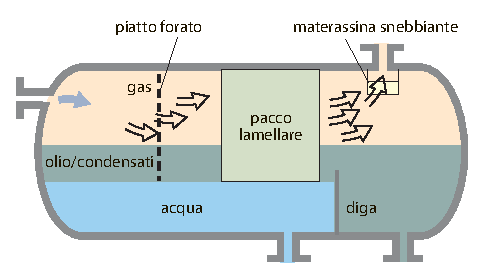
\includegraphics[width=.55\textwidth]{fig/impianti/separatori/trifase.eps}  \label{fig:trifase-interno}} \qquad
    \subfloat[][Dettaglio del pacco lamellare.]
    {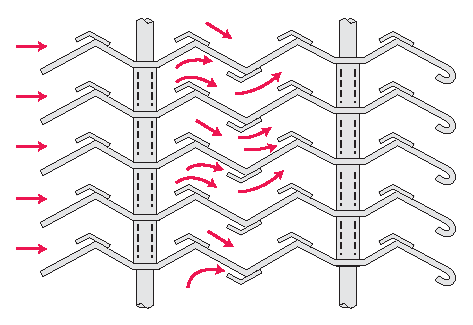
\includegraphics[width=.35\textwidth]{fig/impianti/separatori/pacco-lamellare.eps} \label{fig:pacco-lamellare}} 
\caption{Separatore trifase e del pacco lamellare \parencite{bianco2005impiantiolio}.}
\label{fig:trifase}
\end{figure}

\subsection{Scambiatori di calore}
Numerose sono le tipologie di scambiatori impiegati nell'industria del gas naturale. \\
I più semplici sono gli scambiatori a fasci tubieri e mantello (\textit{shell-and-tubes}, \figref{fig:tubieri}), dove il dispositivo viene attraversato dalle due correnti sul "lato mantello" e sul "lato tubi". Lo scambiatore a fasci tubieri garantisce ottime performance grazie all'estesa superficie di scambio di cui è dotato.

\begin{figure}[htbp]
    \centering
    \subfloat[][Sezione trasversale.]
    {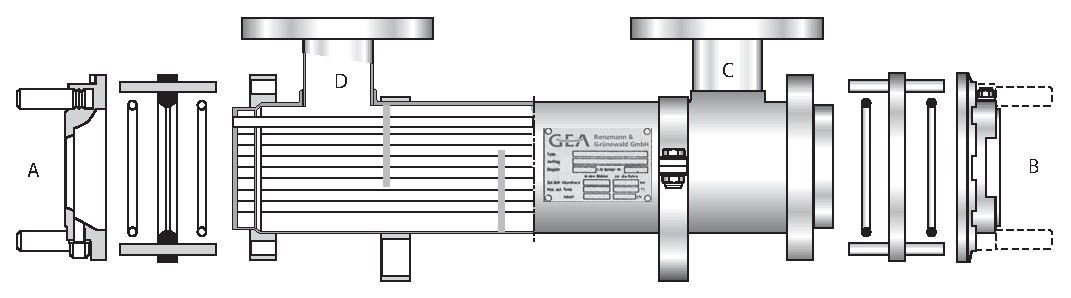
\includegraphics[width=.6\textwidth]{fig/impianti/scambiatori/tubiero-a.eps}  \label{fig:tubieri-a}} \qquad
    \subfloat[][Direzione del flusso all'interno dello scambiatore.]
    {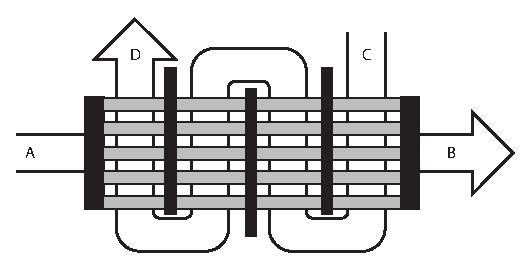
\includegraphics[width=.3\textwidth]{fig/impianti/scambiatori/tubiero-b.eps} \label{fig:tubieri-b}} 
\caption{Scambiatore di calore a fasci tubieri \parencite{guadagni2003prontuario}.}
\label{fig:tubieri}
\end{figure}

Altro dispositivo di scambio termico è lo scambiatore a piastre (\figref{fig:piastre}). Questa tipologia di scambiatore prevede un pacco di piastre rettangolari tutte uguali, ottenute da lamiera per stampaggio secondo diverse forme di corrugazione superficiale. I fluidi lambiscono le piastre attraverso canali che si formano tra esse. Le piastre sono sostenute da un telaio e tenute in pressione da quest'ultimo. Hanno il vantaggio di raggiungere coefficienti di scambio elevati e sono molto flessibili in caso di modifiche progettuali. Inoltre sono molto impiegati in campo off-shore grazie al poco spazio richiesto per l'installazione. Negli ultimi anni hanno preso piede i PCHE (\textit{Plate Compact Heat Exchanger}), un'evoluzione degli scambiatori a piastre, molto richiesti per via della loro ulteriore riduzione di ingombro.\\

\begin{figure}[htbp]
    \centering
    \subfloat[][Piastre dello scambiatore.]
    {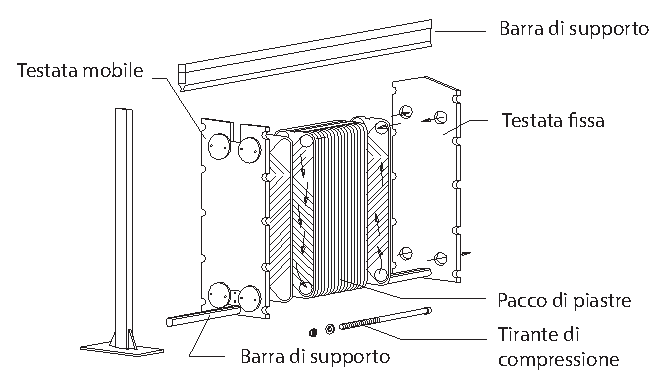
\includegraphics[width=.45\textwidth]{fig/impianti/scambiatori/piatti-1.eps}  \label{fig:piatti-a}} \qquad
    \subfloat[][Ingresso e uscita dei due fluidi.]
    {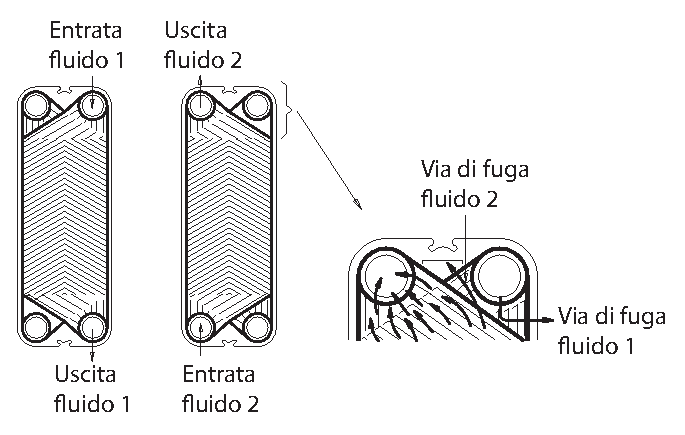
\includegraphics[width=.45\textwidth]{fig/impianti/scambiatori/piatti-2.eps} \label{fig:piatti-b}} 
\caption{Scambiatore a piastre \parencite{guadagni2003prontuario}.}
\label{fig:piastre}
\end{figure}

\subsection{Compressori}
Il compressore è una macchina operatrice che opera su un fluido comprimibile con l'obiettivo di aumentarne la pressione. I compressori possono classificarsi in:
\begin{itemize}
    \item compressori volumetrici o a flusso intermittente;
    \item compressori dinamici o a flusso continuo.
\end{itemize}
 La scelta di un idoneo impianto di compressione si realizza tramite il calcolo del rapporto di compressione richiesto, cioè il rapporto tra la pressione di mandata e quello di aspirazione. Il raggiungimento della pressione finale può avvenire in un unico salto oppure tramite più stadi in serie (\textit{booster}): si parla quindi rispettivamente di compressori monostadio o compressori multipli. In caso di compressione multistadio, il gas naturale viene raffreddato ad ogni step tramite refrigerazione interstadio fino alla temperatura di ingresso.
\paragraph{Compressori volumetrici}
I compressori volumetrici o a flusso intermittente sono macchine che riducono il volume del gas naturale per aumentare la pressione. I compressori volumetrici possono essere classificati a loro volta in alternativi e rotativi.\\
Nei compressori volumetrici alternativi (\figref{fig:compressori-1}) il processo di compressione è realizzato da un pistone che realizza una "corsa" all'interno di un cilindro dotato di valvole di aspirazione e mandata. In una prima fase il pistone porta a compressione il gas all'interno del cilindro che viene poi convogliato alla mandata. Quando il cilindro torna in posizione originale, la riduzione di pressione all'interno del cilindro porta all'apertura delle valvole di ingresso e al ritorno delle condizioni iniziali. Una volta chiuse le valvole di aspirazione il ciclo si ripete. I compressori alternativi sono utilizzati nella compressione di gas naturale per basse portate e alte pressioni.% e la loro alimentazione è a opera di turbine a gas accoppiate direttamente al compressore (hanno un numero di giri analogo). 
Gli svantaggi dei compressori alternativi sono legati ai costi di manutenzione non trascurabili e alla creazione di vibrazioni indesiderate e spinte orizzontali alternate. La \figref{fig:compressori-3} mostra un compressore alternativo a cilindri contrapposti, spesso usato in questo ambito.\\
I compressori volumetrici rotativi spostano e comprimono il gas naturale tramite l'azione di elementi in moto rotatorio. Nell'ambito del trattamento del gas naturale sono impiegati compressori volumetrici rotativi a vite (\textit{rotary screw}, \figref{fig:compressori-4}) costituiti da due rotori accoppiati, di forma elicoidale, che ruotano comprimendo e spostando allo stesso tempo il gas. L'efficienza della macchina dipende in gran parte dai giochi tra i due rotori. I compressori a vite sono utilizzati per gas a basse pressioni, permettono di raggiungere alti rapporti di compressione con un singolo stadio e il loro utilizzo è ormai consolidato negli impianti frigoriferi. 
\paragraph{Compressori dinamici}
I compressori dinamici sono macchine a flusso continuo in cui la compressione si realizza accelerando l'aria quando questa passa attraverso un un elemento rotante ad alta velocità. L'energia cinetica acquisita si trasforma in energia di pressione in parte nell'elemento rotante e in parte in un diffusore statico a valle della girante. I compressori dinamici possono essere centrifughi o assiali.\\
Nei compressori centrifughi (\figref{fig:compressori-5}) il gas viene accelerato in una girante e il flusso principale ha direzione radiale. Questi compressori possono essere monostadio o multistadio (\figref{fig:compressori-6}) e possono gestire portate di gas elevate con notevole flessibilità e mantenendo la pressione di mandata costante.\\% I compressori centrifughi sono le macchine più diffuse nell'industria del gas naturale e hanno come unico limite la portata minima di aspirazione e la macchina motrice più utilizzata è il motore elettrico.\\
I compressori assiali provocano l'accelerazione del gas tramite un rotore palettato e il flusso principale acquisisce direzione assiale. Questi compressori sono impiegati soprattutto per la compressione dei fluidi frigoriferi abbinati alla liquefazione dello stesso.

\begin{figure}[htbp]
    \centering
    \subfloat[][Schema del compressore volumetrico alternativo.]
    {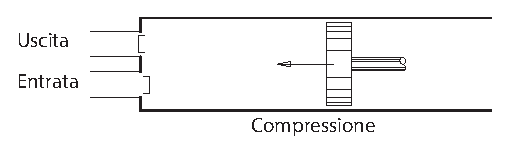
\includegraphics[width=.4\textwidth]{fig/impianti/compressori/compressori-1.eps}  \label{fig:compressori-1}} \quad
    \subfloat[][Schema di compressore rotativo a palette.]
    {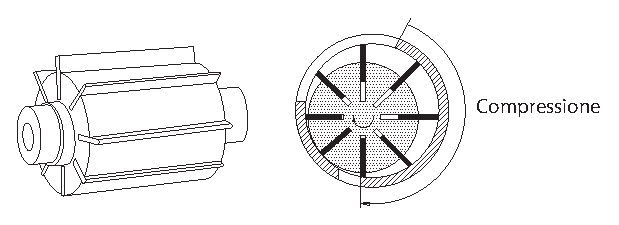
\includegraphics[width=.4\textwidth]{fig/impianti/compressori/compressori-2.eps}  \label{fig:compressori-2}} \\ \qquad\subfloat[][Compressore alternativo a cilindri contrapposti.]
    {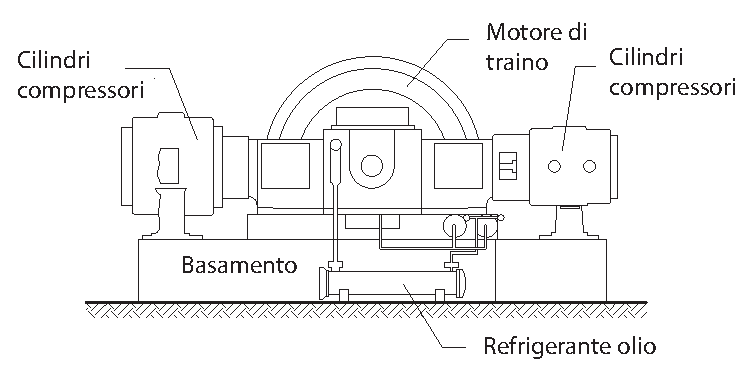
\includegraphics[width=.4\textwidth]{fig/impianti/compressori/compressori-3.eps}  \label{fig:compressori-3}} \quad \qquad\subfloat[][Compressore a vite.]
    {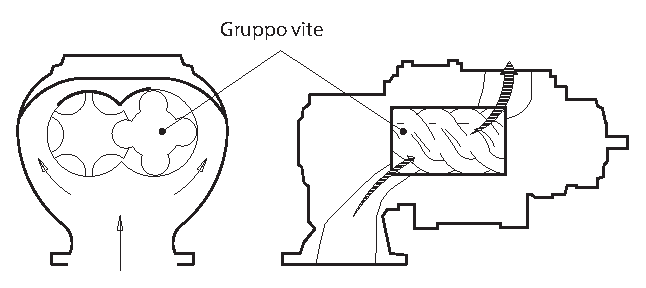
\includegraphics[width=.4\textwidth]{fig/impianti/compressori/compressori-4.eps}  \label{fig:compressori-4}} \\ \qquad\subfloat[][Compressore centrifugo monostadio.]
    {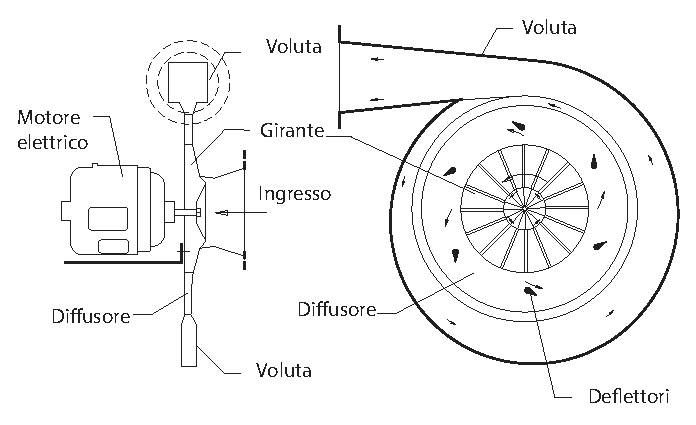
\includegraphics[width=.4\textwidth]{fig/impianti/compressori/compressori-5.eps}  \label{fig:compressori-5}} \quad \qquad\subfloat[][Compressore centrifugo multistadio di processo.]
    {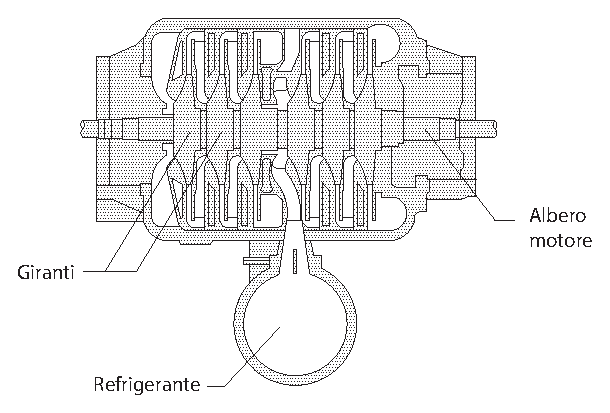
\includegraphics[width=.4\textwidth]{fig/impianti/compressori/compressori-6.eps}  \label{fig:compressori-6}} 
\caption{Compressori \parencite{guadagni2003prontuario}.}
\label{fig:compressori}
\end{figure}

\subsection{Espansori}
Gli espansori più comunemente utilizzati in questo ambito sono le turbine a impulso radiale e le turbine assiali. Le turbine a impulsi radiali sono largamente utilizzate e solitamente queste macchine sono molto compatte. Hanno come unico svantaggio il rapporto di espansione limitato, al fine di mantenere un rendimento elevato. Le turbine assiali invece sono impiegate per potenze elevate e portate di gas rilevanti. L'impiego degli espansori non è oggi una prima scelta nel trattamento del gas naturale ma è un ottima alternativa nel campo della refrigerazione. Al contrario dei sistemi tradizionali (a effetto Joule-Thomson o refrigerazione meccanica), gli espansori sono macchine semplici e compatta e in alcuni casi non richiedono l'impiego di potenza esterna al ciclo.

\subsection{Impianti frigoriferi}
Molti processi di trattamento del gas si basano sulla refrigerazione. Il ciclo frigorifero tramite refrigerazione meccanica (\figref{fig:frigorifero}) si realizza tramite la condensazione di un fluido (solitamente freon) in pressione, il quale viene poi fatto espandere nell'evaporatore (\textit{chiller}) attraverso una valvola. All'uscita dall'evaporatore il fluido refrigerante riportato alla pressione originaria tramite un compressore per poi tornare in fase liquida tramite il condensatore. Il fluido refrigerante è scelto in base alla temperatura di evaporazione che si intende raggiungere. Spesso il ciclo frigorifero può svilupparsi in più stadi, nel caso in cui si vogliano raggiungere temperature molto basse.

\begin{figure}[htbp]
    \centering
    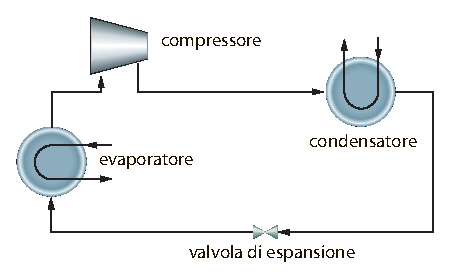
\includegraphics[width=.5\textwidth]{fig/impianti/frigorifero.eps}
    \caption{Refrigerazione meccanica \parencite{bianco2005impiantigas}.}
    \label{fig:frigorifero}
\end{figure}

Tutti i processi descritti in questo capitolo fanno riferimento al trattamento del gas, per poi essere immesso nella rete nazionale. Nel trasporto di gas tra i campi di produzione e le centrali di trattamento non si necessitano di processi di abbattimento spinti delle sostanze associate. In generale le aree pozzo sono dotati di abbattitori per la separazione gravimetrica dell'acqua e sistemi di inibizione di idrati, che consistono nel riscaldamento del flusso gassoso oppure nell'iniezione di glicol in condotta. L'acqua rimane quindi presente del flusso gassoso e può accumularsi negli avvallamenti della condotta, generando così una contropressione. Le cadute di pressione nel trasporto di un fluido in condotta non permettono di operare in modo adeguato e si cerca di diminuire il valore di contropressione tramite diverse soluzioni tecniche. In campo industriale vengono impiegati degli scovoli o pig, dispositivi cilindrici o sferici per pulire, ispezionare e misurare le condotte. Nel prossimo capitolo saranno trattate le diverse tipologie di scovolo e le procedure di piggaggio di una condotta in pressione.
%Come detto in precedenza, il trattamento provvisorio non prevede la totale rimozione dell'acqua dal gas naturale. Di conseguenza nel trasporto del gas naturale in centrale l'acqua può accumularsi negli avvallamenti della condotta, generando così una contropressione. Le cadute di pressione nel trasporto di un fluido in condotta non permettono di operare in modo adeguato e si cerca di diminuire il valore di contropressione tramite diverse soluzioni tecniche. In campo industriale vengono impiegati degli scovoli o pig, dispositivi cilindrici o sferici per pulire, ispezionare e misurare le condotte. Nel prossimo capitolo saranno trattate le diverse tipologie di scovolo e le procedure di piggaggio di una condotta in pressione